\chapter{Data Acquisition and Analysis}

\section{Travel Survey of Residents of Canada}

\subsection{Introduction}
The Transport Survey of Residents of Canada (TSRC) is a monthly, cross-sectional survey collected by Statistic Canada to measure the volume, characteristics and economic impact of domestic travel. The survey provides a large quarterly sample of performed trips within Canada, along with socio-economic data and the activities and expenditures performed on each trip. Results are released yearly, with the data available at a monthly temporal resolution. 

The TSRC was designed to measure the size and economic impacts of Canada's domestic tourism industry. It was first performed in 2005, and replaces the Canadian Travel Survey. In 2011, the survey was redesigned to bring the questionnaire more in line with the World Tourism Organisation guidelines, and align the recorded activities with the International Travel Survey (ITS). 

The TSRC acts as the main data source for the estimation and calibration of the destination choice model presented by this Thesis. Hence, this section provides an overview of the aspects of the TSRC and its design that relate to the development of a destination choice model. In particular, the methodology behind the survey is discussed, and the relevant variables and weightings available in the resultant microdata are highlighted.

\subsection{Method}
The survey is performed as a voluntary supplement to the compulsory Labour Force Survey (LFS). The LFS is a mandatory household survey of around 54,000 households to measure employment, and has a 90\% response rate. The LFS sample consists of the entire civilian, non-institutionalized population over 15 years of age. A sub-sample of these households is selected to answer the TSRC, excluding residents of the Yukon, the Northwest Territories and Nunavut and people living on Native Reserves. A respondent is randomly selected from the household and asked to complete the travel survey. The survey is a computer-assisted telephone interview (CATI) available in both of Canada's official languages, English and French. 15 minutes are allocated for each respondent, with as many trips being collected as possible in that time.

\subsection{Data}
\label{section:tsrcdata}
\subsubsection{Spatial Resolution}
All spatial data points, namely those for home location, trip origins and destinations and stopovers are provided in the microdata at three resolutions, Province or Territory, Census Division, and Census Metropolitan Agglomeration (CMA). Canada is made up of ten provinces and three territories, the largest of which is Ontario, the focus of this thesis. 

Census Divisions are the next largest geographical area in Canada. Census Divisions represent groups of neighboring municipalities combined to aid regional planning and the provision of common services. After the provinces and territories, they are the most stable spatial unit. They were last modified for the 2011 census, and therefore are consistent between each TSRC dataset since the revised version was introduced. In most provinces and territories, these census divisions are defined in legislation, however in Newfoundland and Labrador, Manitoba, Saskatchewan, Alberta, Yukon, Northwest Territories and Nunavut, provincial or territorial law does not provide for these administrative geographic areas. In these cases, the census divisions are allocated by Statistics Canada.

Census sub-divisions are the next smallest geographical area, representing individual municipalities. These are recorded as part of the survey, however are not available in the TSRC microdata. The finest level of aggregation available is that of the Census Metropolitain Areas (CMA) and Census Agglomerations (CA). CMAs and CAs represent certain clustered areas of population around an urban core. More specifically, to be defined as a CMA, an area must have a total population of at least 100,000, with half of those living in the core urban area. CAs, which related to CMAs but require a core population of only 10,000, are not recorded in the TSRC data. 

Since CMAs do not topographically cover the whole Canadian study area, but only identify particular dense urban areas, census divisions are the most detailed resolution available for consistent use when working with the TSRC data. CMA’s are only recorded for 51.5\% of trip origins, and 48.3\% of trip destinations. However, CMA's can be used to better allocate trips to transport zones in urban areas, as discussed in section (CITE).

\subsubsection{Error Detection and Imputation}
The computer-assisted nature of the survey allows for real-time error detection and consistency checking during the interview process. One example is that the program will inform the interviewer if the number of nights recorded for a trip does not match the number of nights recorded in various types of accommodations. ‘Don’t Know’ and ‘Refused’ are also valid options for many questions, to prevent false answers been recorded. Sanity checks against extreme values are also performed, and the coding of geographical areas is mostly performed automatically.

Two forms of imputation are performed for the survey, for trip details and expenditure amounts respectively. Since the survey only allows 15 minutes for the recording of trip details, the details of non-selected trips are imputed from other trips recorded for that resident. This imputation process is multi-staged, and is performed per respondent. A donor pool of trips is selected that are similar to the non-selected trip. A distance function is then used to select the closest donor-trip to the recipient, and the detailed variables (activities, expenditures, etc) are copied over to the recipient trip.

\subsubsection{Weighting}
The weighting of records is particularly important when working with survey data. They allow the researcher to scale up the results for a sample to build an accurate representation of population, taking into account under- and over- represented groups within the survey. In total, four weightings are provided for the TSRC, with two relating to trip avriables:
•	full-sample person weights
•	first-month person weights
•	person-trip weights
•	trip weights

As the TSRC sample is based on the LFS survey, person weights are applied from the LFS and recalibrated to reflect subsampling, non-response, and known control groups. 

After the 2011 redesign, respondents are asked about same-day trips that ended in the previous month, but overnight trips that ended in the previous two months. This means that effectively only half the sample is asked about same-day trips. To account for this, two weights are provided for each person record. A first month weight, that can be used for any person variable, and a second "full sample" weight that can be applied to person characteristics and overnight travel variables.

The person-trip weight, used to estimate trip volume, is then calculated by accommodating for identical trips, declared and reported trips, missing data and non-response. These weights are treated for outliers and recall bias. In calculating the person-trip weight, the person weight is also multiplied by the number of identical trips that this trip represents. The person-trip weight (WTEP) can be used against all socio-economic characteristics, as well all trip and visit variables, excluding expenditures. Trip weight (WTTP) is then calculated by dividing the number of household members that went on the trip, is only used to calculate expenditures, and as such is not relevant to the model design. 

\subsection{Microfile Format}
The results from the TSRC are provided as yearly collections, separated into individual files for persons, trips and visits. The survey results are provided as fixed with delimited .dat files. A code book and data dictionaries are provided to decode the values stored in each line. The schema for encoded variables such as province are consistent across files and years (i.e. Ontario is always coded as 35), meaning that once read from the correct position on a line, values don't need to be decoded before being compared with each other. 

Each person record is associated with one or more trips. Not all persons recorded in the person microdata necessarily have a trip recorded for a particular time period, as the survey records the travel behavior of both travelers and non-travelers.

Each recorded trip record has at least two associated visit records, or more if intermediate overnight stops were recorded. Visits are classified into two types, origins or destination/airport. Each Trip has one origin visit record, and at least one destination record. Where the main mode of travel for the trip is "Air", two or more airports are specified as visit records, along with the 3-digit airport code for the respective Canadian airport. The survey codebook notes that these airport records may be adjusted to protect respondent privacy.

\subsubsection{Trip Datafile}
Trips covered by the TSRC include same-day trips of more than 40km and overnight trips with at least one night in Canada. Domestic same-day and overnight trips are recorded in full. International trips with no nights in Canada are not recorded in the TSRC. For trips with an overnight destination, but some nights in Canada, only the domestic portion of the trip is recorded, with the point of departure from Canada recorded in the MDxxx variables for trip destination. The TR\_D11 variable records the number of times this trip was performed in the reference month, and must be taken into account when estimating trip frequencies.

Socio-economic variables for the traveler are recorded for each trip record; namely age, gender, education level, employment status and income. The number of household members who participated on the trip is also recorded.

Trip purpose is  recorded at two categorical levels. In the first, purposes are split into four options:
\begin{itemize}
\item Holidays, leisure or recreation
\item Visit friends or relatives
\item Business - All business and work related trips, except routine travel which is a regular part of the job
\item Other - All trips for other reasons except regular household chores
\end{itemize}

\subsubsection{Visit Datafile}
The visit data file provides a stops performed on each trip, which can be linked to the relevant trip by the Public Use Microdata File Number (PUMFID) and the Trip Identification Number (TRIPID). Each trip has at least two visits associated with it, an origin and a destination visit, differentiated by the VISRECFL variable. The AIRFLAG variable is used to identify visit records that refer to an airport entry or exit. 

If a location is visited twice during a single trip, only one visit is recorded for that location. The visits are not guaranteed to be recorded in the chronological order of visitation, even though the visits are collected in chronological order during the survey process. This lack of order prevents the visit records from being used model trip chaining, as discussed in section (CITE).

\subsection{Season of Travel}
Canada has starkly contrasting seasons which influence travel choices of residents. The TSRC provides the month of travel for each trip, and these are aggregated into two seasons, designed to highlight the impact of winter conditions on long distance travel behavior. For this thesis, the months from November to March are considered winter, with the rest as summer. With this classification, summer covers 7 out of 12 months of year, or 58.4\%. Table~\ref{table:season-split} shows how leisure and visit trip counts occur disproportionately in the summer months. The $P$ value indicates the probability that this result is not by chance.

% Table generated by Excel2LaTeX from sheet 'Sheet1'
\begin{table}[H]
\centering
\caption{Seasonal split of TSRC trips}
\label{table:season-split}
\begin{tabular}{p{4.07em}cccc}
\toprule
\multicolumn{1}{r}{} & \multicolumn{1}{p{5em}}{Summer} & \multicolumn{1}{p{4.645em}}{Winter} & \multicolumn{1}{p{3.93em}}{Summer \%} & P  \\ \midrule
Business & 11,750 & 8,641  & 57.62\% & 0.02 \\
Leisure & 52,639 & 19,774 & 72.69\% & 1.00 \\
Visit & 61,630 & 39,856 & 60.73\% & 1.00 \\ \bottomrule
\end{tabular}%

\end{table}


It is self explanatory that destination choice should depend on seasonal factors. The example of winter sports is a prime example. Winter sports is an activity that people willing travel long distances for. In 2014, TSRC respondents reported participating in winter sports in 4\% of overnight trips, and 2\% of same day trips. These trips naturally only occur in the winter months, at certain destinations. Section~\ref{section:season-estimation} demonstrates how the consideration of seasons can improve the model. 

\section{Filtering of Trip Records}
For the model input, the TSRC trip records from 2011 to 2014 were collated together, giving 220,512 trip records. Not all these trips were relevant to the estimation of the destination choice model. Firstly, records were removed where:
\begin{itemize}
\item Either an origin or destination is not stated
\item The trip purpose is not leisure, visit or business
\item A distance is not recorded
\item The mode is recorded as air and the destination and origin airports are identical
\end{itemize}

The TSRC trip files provide trip records not just for Ontario, but for all of Canada. However, as a model for Ontario, we are only concerned with the following categories of trips that influence travel in Ontario:
\begin{itemize}
\item Internal trips within Ontario - Internal (II)
\item Trips entering Ontario - Incoming (EI)
\item Trips leaving Ontario - Outgoing (IE)
\item Trips that cross Ontario - External (EE)
\end{itemize}

Any trips that didn't fit one of these categories is also excluded from the trip dataset used to estimate the destination choice model. Internal, incoming and outgoing trips don't need to be filtered, and all trips in these categories are retained in the trip set. External trips, on the other hand, are filtered to remove trips that don't cross Ontario. Excluding such external trips is important to make sure that the estimated model reflects the behavior of travel in Ontario, which could be different to the behaviors in other provinces. 

\begin{figure}[H]
\centering
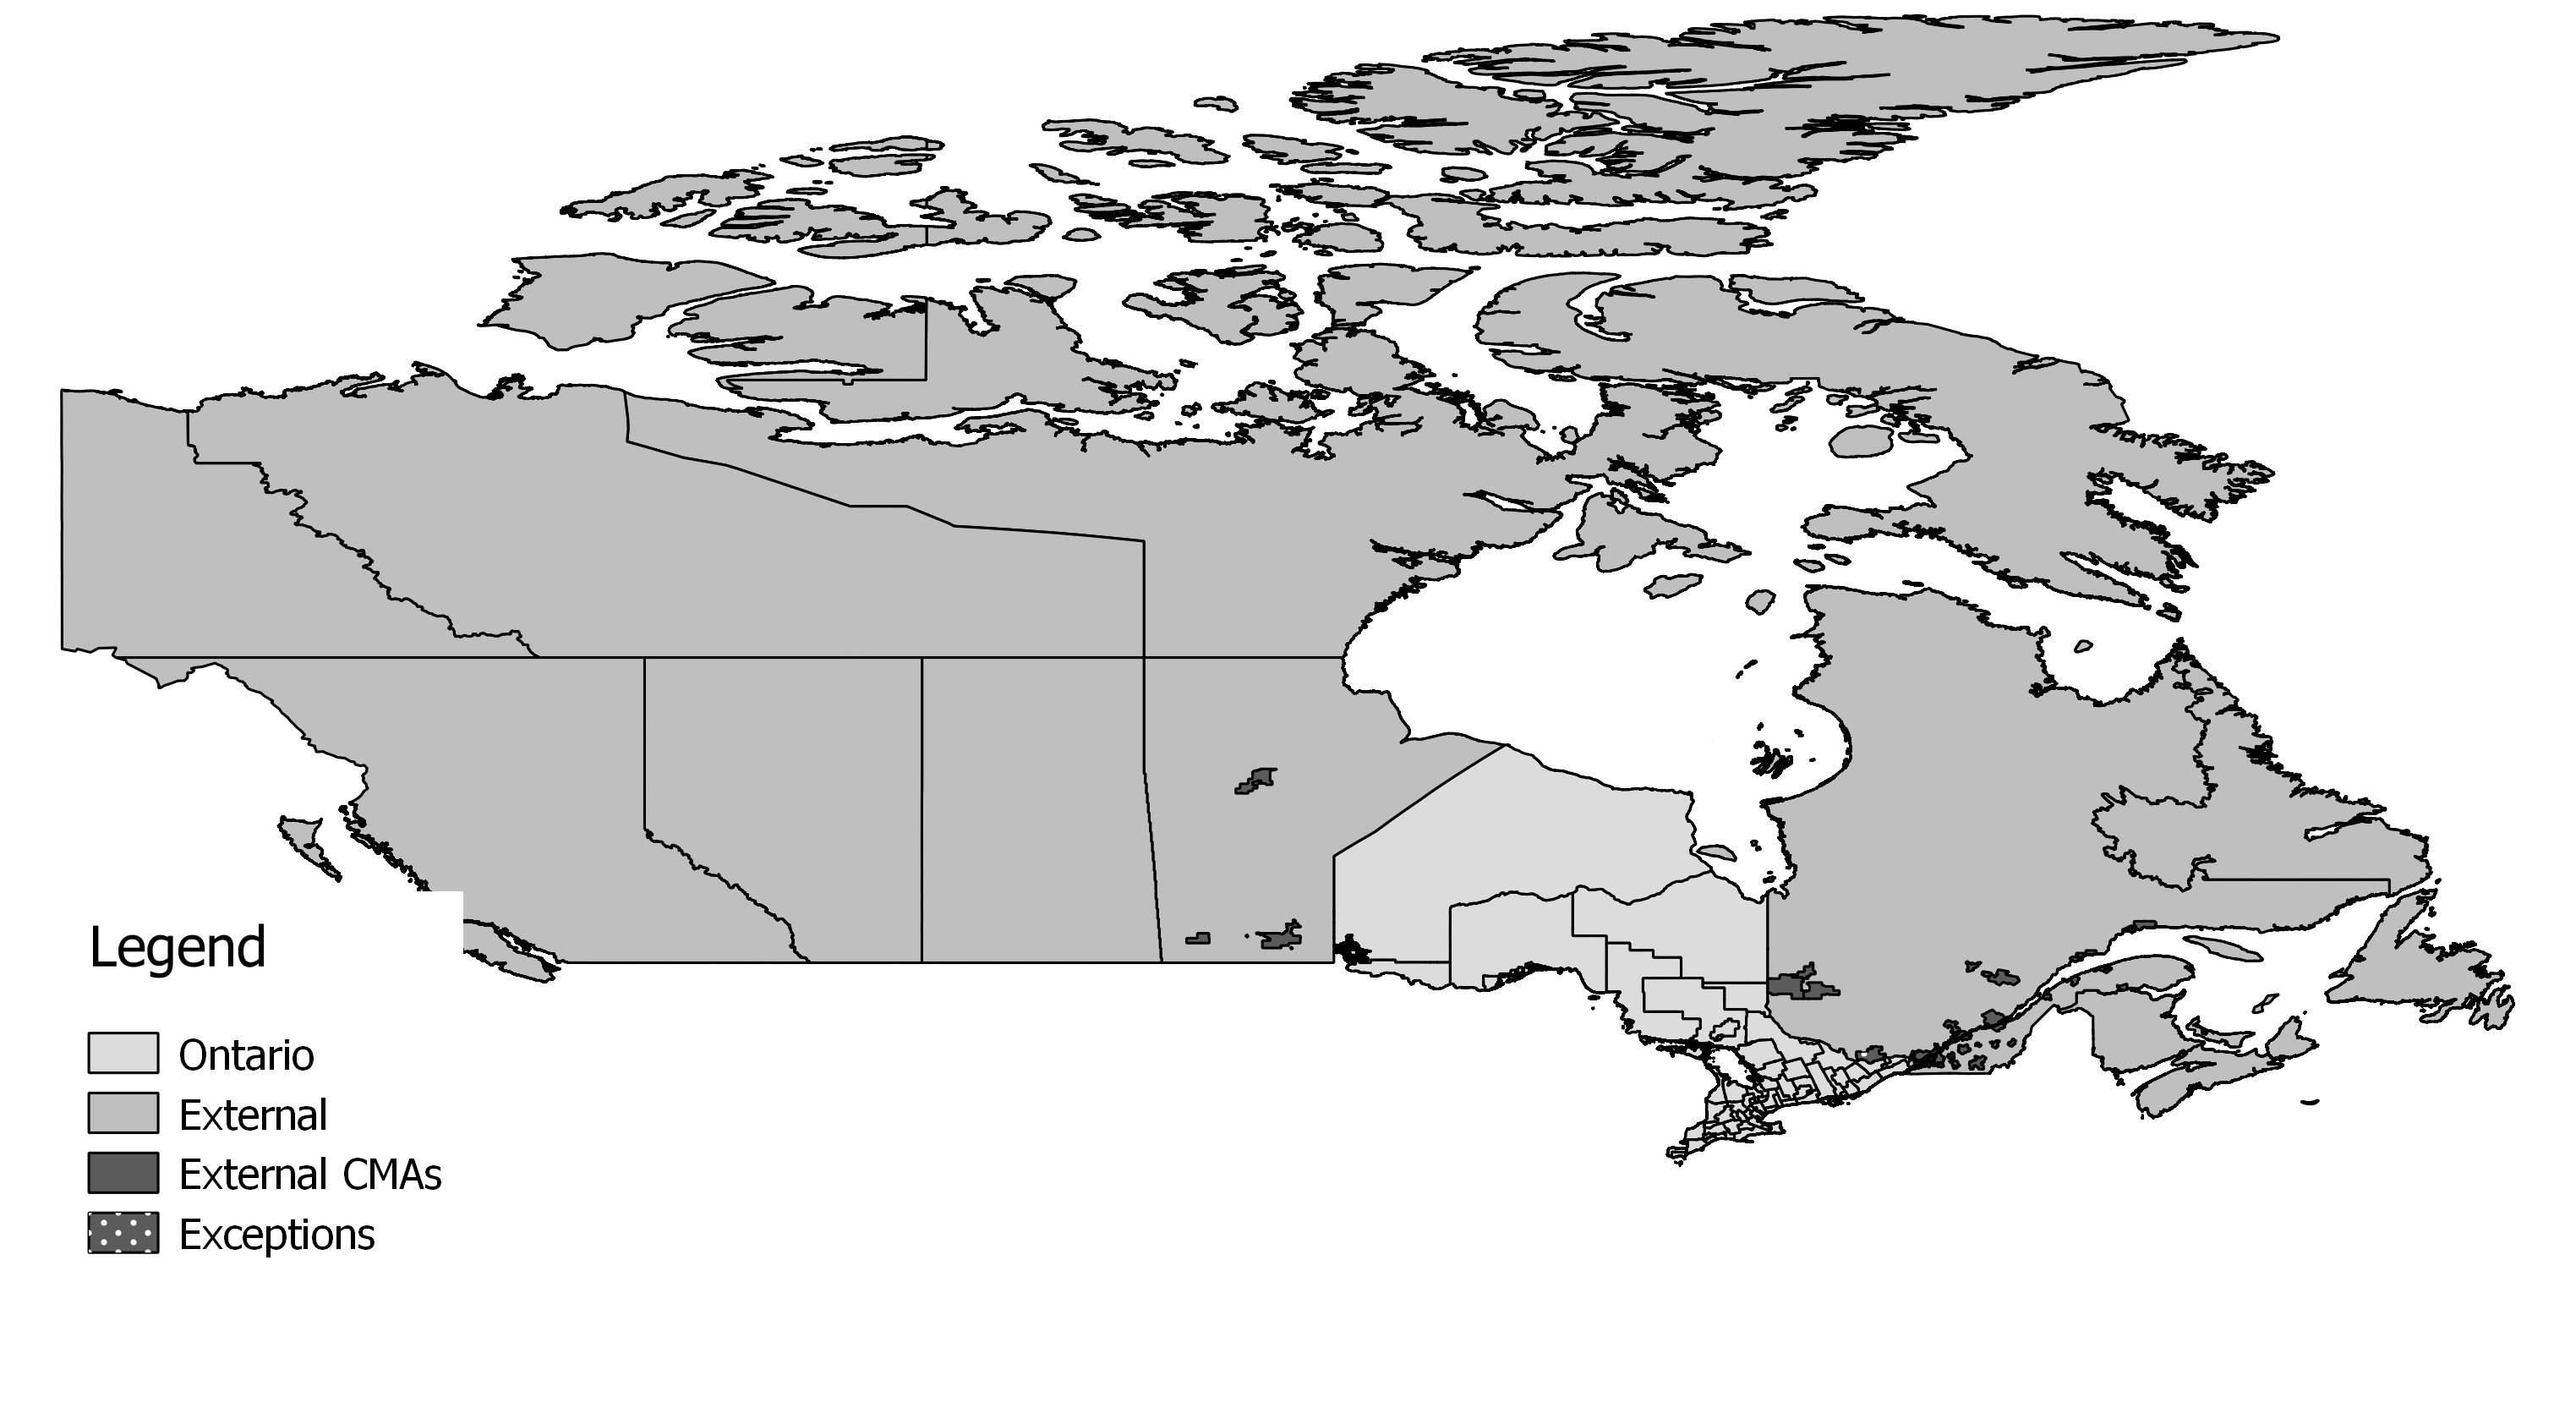
\includegraphics[width=\textwidth]{ontario_land_bridge}
\caption{Dividing external zones into east and west}
\label{fig:bridge}
\end{figure}

The unique geography of the Canadian provinces greatly restricts the number of external origin-destination pairs that need to be considered when excluding unwanted external trips. Ontario acts as land bridge between the eastern and western parts of Canada, see figure~\ref{fig:bridge}, dividing the external zones into two groups, east and west. Trips originating in one group and arriving in another have to pass through Ontario. And the converse in true for trips within a group. Hence all trips that don't go between east and west can be removed. There are two zones which are the exception to this, zones 85 and 117 in western Quebec. Journeys between these zones and other zones in Quebec may pass through Ontario. For example, figure~\ref{fig:exception85} illustrates a journey from Gatieau, Quebec to Montreal Airport takes around 2 hours when passing through Ontario, and 2 hours and 30 minutes otherwise. Trips between these two exception zones and all other zones in Quebec are therefore retained. 

\begin{figure}[H]
\centering
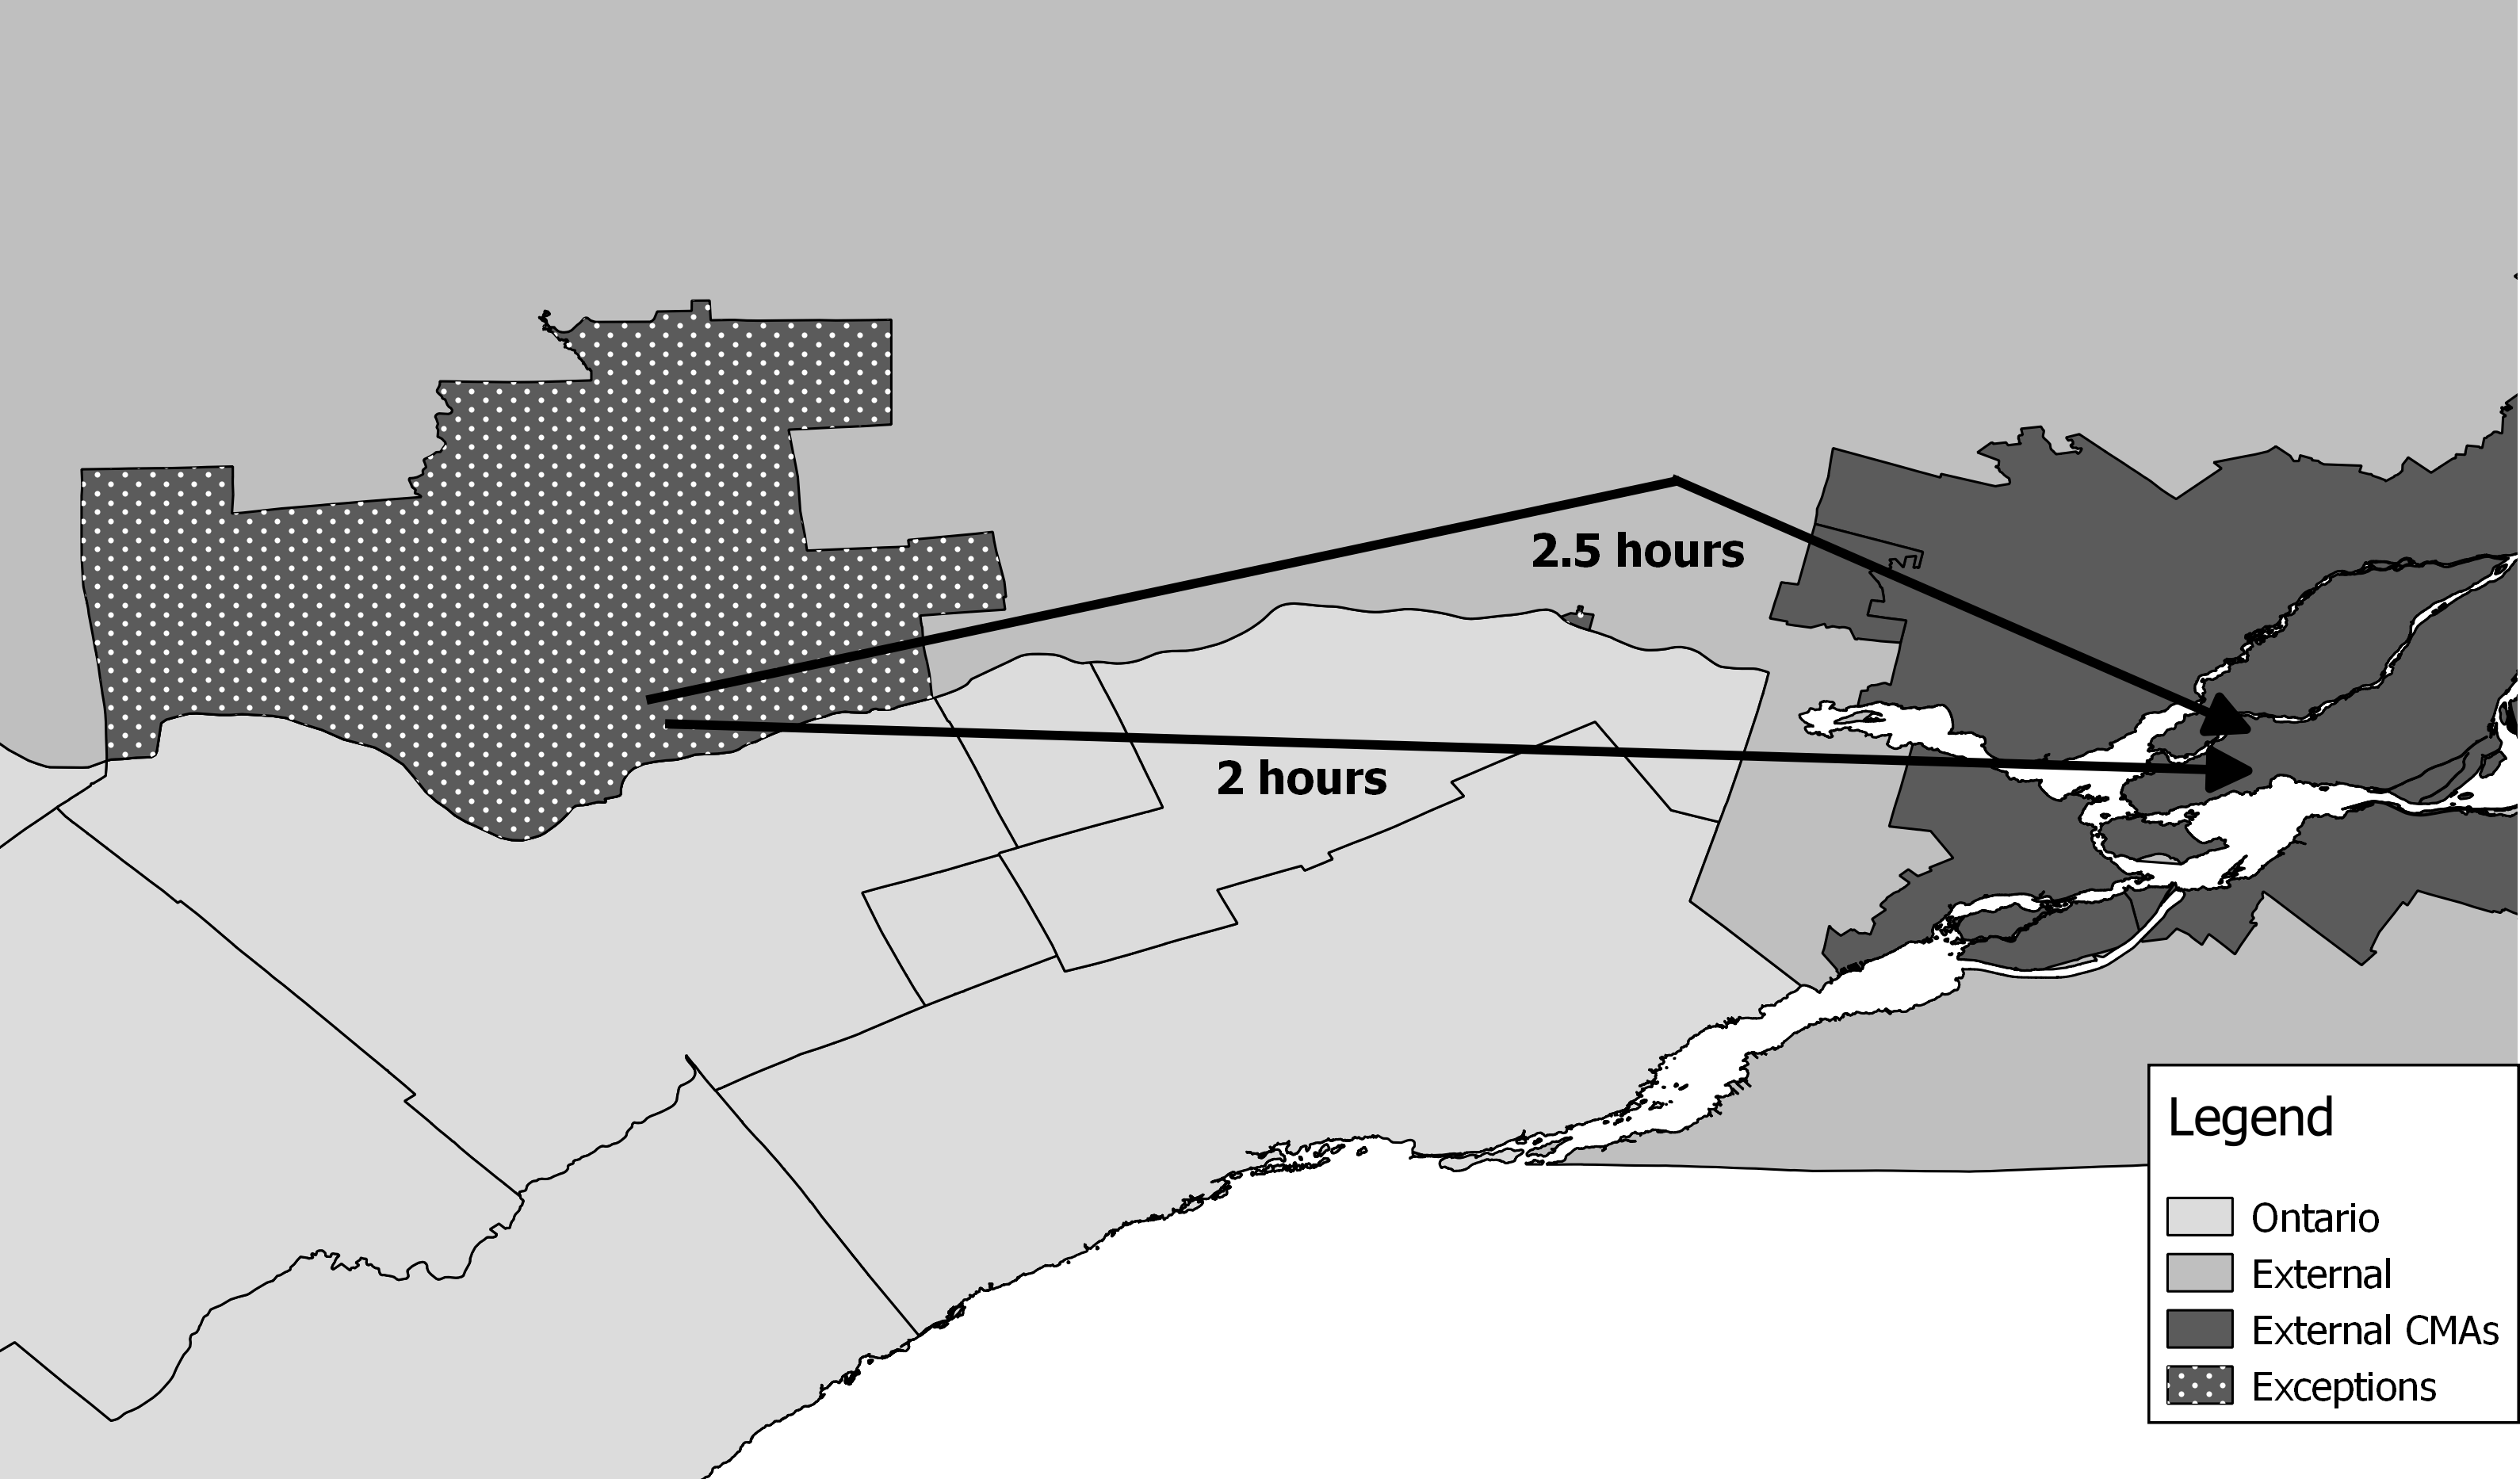
\includegraphics[width=0.7\textwidth]{zone_exception_85}
\caption{An example of an external origin-destination pair that passes through Ontario}
\label{fig:exception85}
\end{figure}


Figure~\ref{fig:distance} illustrates how our the trip distribution of the estimated trips fits the observed distribution much better after undesired external trips are removed. In total 69,328 individual trip records remain from the TSRC dataset for model estimation, representing 40,177,841 weighted trips.

\begin{figure}[H]
\centering
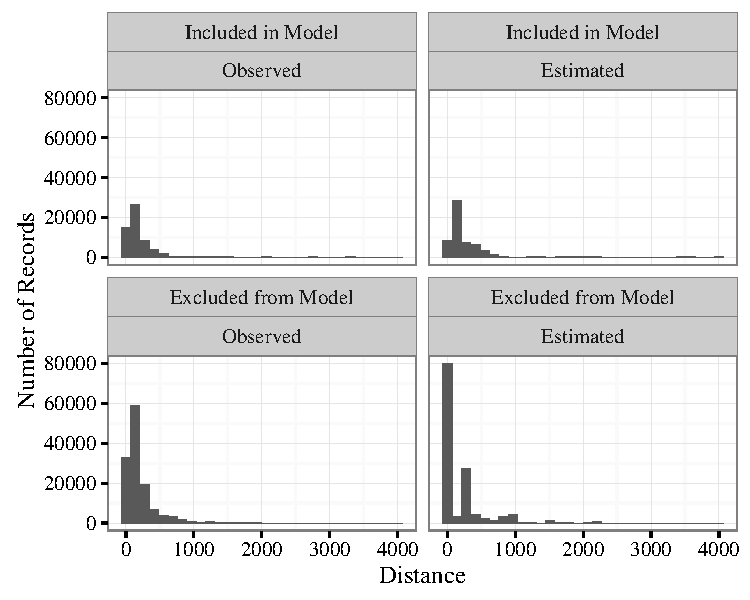
\includegraphics{est_vs_obs_distance}
\caption{Estimated vs. Observed Trip Distance}
\label{fig:distance}
\end{figure}

\section{Zone System}
To avoid confusion throughout the rest of this thesis, the reader should be aware that there are two zone systems considered in the following chapter.
\begin{itemize}
\item \textbf{TAZs}, or traffic analysis zones, are the zones provided for the project, representing the final spatial resolution of the transport model.
\item \textbf{Zones}, are the zones representing the destinations in the destination choice model, referred to collectively as the \textit{zone system} in the remainder of this thesis.  
\end{itemize}

This chapter discusses the definition of the choice set of alternatives for the destination choice model. Numerous factors need to be considered when designing the choice set. Firstly, The sample size of the data available to estimate the model coefficients is an important restraint. With a small sample set relative to the size of the destination choiceset, not enough records are available to calculate the parameter coefficients with high confidence. The size of the choiceset needs to be considered. Large destinations choice sets lead to very long computation times when estimating the model coefficients. A balance needs to be found between the detail represented in the choice set, and the computability and validity of the coefficients.

For this particular destination choice model, a zone system was already provided, consisting of 6671 Traffic Analysis Zones (TAZ). The TAZs can be grouped into 4 categories; 6495 internal zones for Ontario, 48 and 121 external zones representing the rest of Canada and North America respectively, and 7 zones for remaining world-wide destinations. As this thesis is only concerned with domestic travel within Canada, only the Internal zones for Ontario, and 48 external zones within Canada are considered. The external zones are not modified as TSRC origins and destinations are directly translatable to the external zones.

For the Internal zones (TAZs) within Ontario are allocated using a gradual raster based zone approach, based on the method presented by \textcite{moeckel2015gradual}. The 6495 generated TAZs vary in size from $0.879 km^2$ to $3600km^2$, with smaller cells defined for more populous areas, and larger cells for regional areas. The gradual zone system is designed on the premise that it is desirable to have larger zones in rural areas where there is less population, and hence, less activity. This method reduces the number of TAZs, and hence, the complexity of the model, while only removing detail where it is least required. 

However, the TSRC trip origins and destinations don't match this custom zone system for Ontario, being only available at a much broader resolution. For this thesis, a zone system is designed based on the TSRC spatial resolution for the design of a destination choice model. The allocation of trips to the TAZ level will be performed at a later stage in the transport model, and the proposed method is discussed further in section~\ref{section:implementation}.


\subsection{Defining a zone system for Ontario based on the TSRC data}
As discussed in \ref{section:tsrcdata}, provinces and census divisions cover the national study area completely. hence as a first step, the zones are defined by the census divisions comprising Ontario, of which there are 49. However, even in rural areas, the TAZs are much smaller than the size of a Census Division. When the zone system is defined purely using the Census Divisions within Ontario, over 50\% of Census Divisions have more than 75 TAZs, with a large spread (see figure~\ref{fig:zoning}. 

Although CMAs are defined only for selected urban areas of Canada, they can be considered alongside the CDs when allocating zones to improve the spatial resolution of the zone system. The concept of a CMA aligns closely with the objective behind the gradual raster cell size of the provided zone system for Ontario. CMAs identify areas of denser population around an urban core that may be of particular significance to geographers and modellers. By simply including CMAs as zones in the aggregated zoning model, the number of zones is increased to 57, allowing trip origins and destinations in urban areas to be more accurately assigned during disaggregation to TAZs. As seen in figure~\ref{fig:zoning}, this significantly lowers the mean number of TAZs per zone, and also reduces the spread of values, indicating a much improved zone system. 

This approach has one drawback, as a large outlier, representing the Toronto CMA is now observable, consisting of over 2000 TAZs. This outlier corresponds to the CMA of Toronto, the most populous in Ontario, both a very large generator and attractor of trips. In 2014, Toronto represented 13.4\% and 10\% of trip origins and destinations respectively. It should be clear that this is a very undesirable occurrence. While it is hard to say whether this outlier would significantly affect the destination choice model, it would regardless provide significant challenges when allocating trips to individual TAZs, affecting the overall quality of the model. It is worth noting briefly that the choice of zone system can have cascading effects throughout the whole transport model, which need to be considered during its creation.

\begin{figure}[H]
\centering
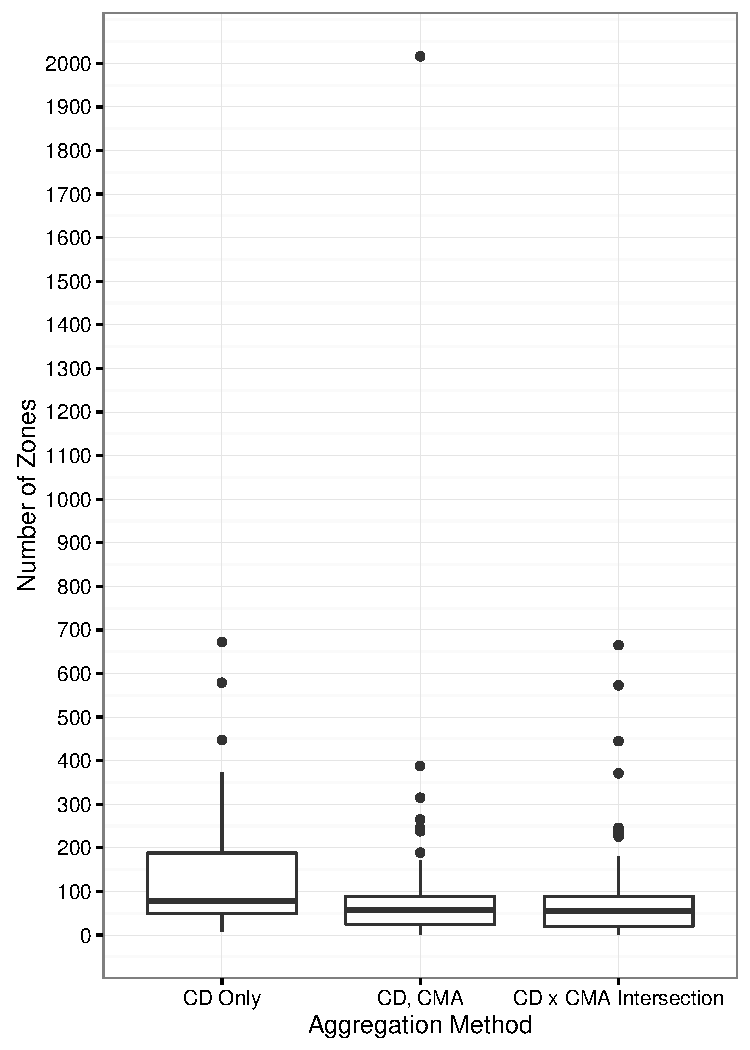
\includegraphics[width=0.5\textwidth]{zoning_methods}
\caption{Different methods of aggregating internal zones to match the TSRC spatial resolution.}
\label{fig:zoning}
\end{figure}

This lone outlier was not present when only the CDs were considered as destination alternatives. Since CMAs often overlap multiple CDs, rather than simply including CMAs and CDs independently, we can overlap the CDs and CMAs to fully reflect the number of destination choices available in the TSRC data. This is done as followed; the area of each CD that does not intersect with a CMA is selected as a zone. Then, each unique combination of CMA and CD is recorded as a new zone. An example of this process is shown in figure (CITE). This process gives us 69 zones for Ontario, at 41\% increase over the simplest approach that only considers CDs.

Figure~\ref{fig:zoning} illustrates the difference between these methods. When only Census Divisions are used, a significant number of CDs have a large number of assigned TAZs . When the CMAs are considered, the results are clearly better. A lower average number of TAZs per aggregate zone will give better results when trips origins and destinations are disaggregated. Taking the intersection of CDs and CMAs has little effect on most zones, but still improves the overall result in a very significant way. The CMA of Toronto overlaps with 7 separate CDs, and can with this method be divided into seven smaller zones.

This third method has another advantage, in that the a distinction between urban and rural areas is now encoded into the zone system. This will be important in the estimation process as 51.5\% of trips in the filtered TSRC survey originated in a CMA, and 48.3\% had destination recorded as a CMA. Not only is it clear that urban areas are important drivers of long distance travel, but that, interestingly, CMAs are more likely to be origins than destinations.

\section{Aggregating of Zonal Data}
All the data on distances, population and employment was provided at the TAZ level. This section describes how they were allocated to the zone system. The TAZs themselves were assigned to the zone which intersected their centroid. Where the centroid of the TAZ didn't intersect any zones, the first intersecting zone was used. When the TAZ did not intersect with any part of the Canadian census boundaries at all, it was assigned manually to the nearest zone.

Socio-economic variables, namely population and employment were aggregated from the TAZ level to the zone system using a summation.

A distance matrix was provided for the original set of TAZs. It was calculated without congestion using the Canadian road network and intra-zonal travel times were not included. This skim matrix needed to be aggregated to the zone system used in the destination choice model. This was done by taking a distance $d$ between each pair of sub zones weighted by the multiplied populations $p$ of the origin and destination.

$$ d_{ij} = 
\frac{
\sum_{k \in i, l \in j} d_{kl} \cdot p_k \cdot p_l}
{
\sum_{k \in i, l \in j} p_k \cdot p_l
} 
$$

\section{Foursquare}
\label{section:data-foursquare}
Trip distribution models that consider only population and employment have a significant flaw. They fail to account for points of interest (POI), such as National Parks that attract large numbers of people, yet exist in areas of low population and employment. Discrete choice modeling provides the opportunity to incorporate parameters that reflect these drivers of travel demand. 
	
Leisure travel is a particular case where socioeconomic metrics don't always reflect the attractiveness of a destination. Areas such as as lakes, national parks and ski resorts are popular long distance recreational destinations in the summer and winter respectively, yet have small populations and employment. 
\textcite{simma2001destination} developed a destination choice model for leisure travel in Switzerland that considered many variables of destination attractiveness such as the number of swimming pools, ski area qualities and land use attributes. They found that while
	
The TSRC microfile records the activities performed on each recorded trip and destination visited during a trip. When aggregated by trip destination, these activities give an indication of which zones provide particular attractions such as national parks or ski areas. The number of trips with each recorded activity can also be used to identify the importance of a particular activity for each zone. However, there are two key problems with this approach:

\begin{itemize}
\item When implementing of the model,  The spatial resolution of the TSRC microfile means that the location where an activity was performed can only be determined at a zone level. Another data source is still needed to identify key points of interest such as hospitals and tourist attractions to predict trip destinations at the TAZ level.
\item As a domestic survey, the TSRC doesn't cover the US, meaning a different method would need to be used to identify key attractions across the border.
\end{itemize}	
In this section, we describe how the collection and processing of foursquare check-in data was performed in order to build destination utility variables.

\subsection{Foursquare Venue Search API}
Foursquare collects a wealth of data, on where and when users check-in. Users and their behavior can be tracked over time using twitter as a proxy, however the time-frame for this thesis made this method unfeasible. Instead, the public venue API was used, which is much more limited in its scope, only providing a cross-sectional dataset of POIs within the search area. For a search area and criteria, the API returns a list of venues in JSON format. Each venue record provides the following relevant information:
\begin{itemize}
\item Name
\item Venue category
\item Geo-referenced location
\item Number of unique visitors
\item Number of total check-ins
\end{itemize}

Each request is limited to roughly 1 square degree of longitude and latitude in search area, and only the top 50 venues for that search are returned. A limit of 5000 requests per hour is also enforced. Search results are returned based on the popularity of the venues. How the rank of returned venues is determined by foursquare is not specified. 

The API does not return check-in counts by date, so it can only be used to generate a total metric of activity for each venue, up to the time of the search. For the forecasting of trips to individual venues, this would present a significant obstacle. In this thesis, however, the foursquare metrics are only used for identifying the intensity of activity in zones that may not be reflected in socioeconomic variables. Check-in counts also can not be filtered by origin country or state. This capability would, in a larger model, also allow us to identify U.S. destinations that are commonly visited by Canadian travelers, as opposed to all users of foursquare.

\subsection{Demographic Bias}
While the use of social networks is becoming more ubiquitous throughout the general population, LSBNs such as foursquare still have a particular user demographic, which should be taken into account when working with social network based data. The data retrieved from the foursquare API does not provide any demographic information that can be used to weight the retrieved data.

In this thesis, the potential impact of bias is minimized, as only the intensity of activity for each category in a zone is measured as a variable. There is also no stratification of these variables by age, gender or education level in the model estimation. Such stratification would cause concerns with demographic bias, for example with older groups of travelers. One concern is that certain venue categories could be under-represented in the data, such as aged care services, or those where a check-in might be taboo such as a place of worship. This is considered by grouping venues into broad categories, which are then considered as model parameters.
	
\subsection{Methodology}
To collect the venue data from the Foursquare API, the following procedure was followed:
\begin{enumerate}

\item A developer account was set up which allowed access to the API. The maximum search area allowed is smaller than most external zones, so a search grid of 1 degree raster cells was generated for the study area. 

\item Using the activities specified in the TSRC as a reference, a selection of potentially important venue categories was curated (see table~\ref{table:foursquare_categories}).

\item Each category was mapped to at most 5 main foursquare venue categories, on which the search was performed. This is necessary to exclude venue categories such as ``States \& Municipalities".

\item A python script was written to query the foursquare API for each raster cell and category, returning the top 50 venues, while adhering to the rate limit of 5000 requests per hour. Calls to the api had to be structured as:
\begin{verbatim}
https://api.foursquare.com/v2/venues/search?intent=browse
    &limit=50&sw={sw}&ne={nw}& categoryId={categories}
\end{verbatim}
where 
\begin{itemize}
\item sw, ne are the bottom-left and top-right corners of the search area
\item categories is a comma separated list of venue ids.
\end{itemize}

\item Unique venues were then stored in the PostGIS database, and each tagged with the zone to which it geographically belongs.
\item Two attributes were then calculated for each zone and category; the number of venues of that category in the zone, and the number of check-ins for each category and zone.
\end{enumerate}

The foursquare API provides data at a higher spatial resolution than the TSRC microfile, but without the temporal detail. In table~\ref{table:foursquare_categories}, the number of venues and check-ins per category are presented. In total, 34,041 unique venues and 7,981,458 check-ins were collected for the different categories.

%\afterpage{%
%    \clearpage% Flush earlier floats (otherwise order might not be correct)
%    \thispagestyle{empty}% empty page style (?)
%    \begin{landscape}% Landscape page

% Please add the following required packages to your document preamble:
% \usepackage{booktabs}
\begin{sidewaystable}[]
\centering
\caption{foursquare venue categories}
\label{table:foursquare_categories}

\centering % Center table

% Table generated by Excel2LaTeX from sheet 'Sheet1'
% Table generated by Excel2LaTeX from sheet 'Sheet1'
\begin{tabular}{lrrrrrrr}
\toprule
Search Category & \multicolumn{5}{c}{Venue Categories}  & \multicolumn{1}{l}{Venues} & \multicolumn{1}{l}{Check-ins} \\
\midrule
Medical & \multicolumn{1}{l}{Dentist's Office} & \multicolumn{1}{l}{Doctor's Office} & \multicolumn{1}{l}{Hospital} & \multicolumn{1}{l}{Medical Center} & \multicolumn{1}{l}{Veterinarian} &          6,294  &              586,082  \\
Ski Area & \multicolumn{1}{l}{Ski Area} & \multicolumn{1}{l}{Ski Chairlift} & \multicolumn{1}{l}{Ski Chalet} & \multicolumn{1}{l}{Ski Lodge} & \multicolumn{1}{l}{Ski Trail} &          1,048  &              203,266  \\
Airport & \multicolumn{1}{l}{Airport} & \multicolumn{1}{l}{Airport Gate} & \multicolumn{1}{l}{Airport Lounge} & \multicolumn{1}{l}{Airport Terminal} & \multicolumn{1}{l}{Plane} &          1,882  &          1,919,050  \\
Hotel & \multicolumn{1}{l}{Bed \& Breakfast} & \multicolumn{1}{l}{Hostel} & \multicolumn{1}{l}{Hotel} & \multicolumn{1}{l}{Motel} & \multicolumn{1}{l}{Resort} &          7,268  &          1,502,248  \\
Nightlife & \multicolumn{1}{l}{Bar} & \multicolumn{1}{l}{Brewery} & \multicolumn{1}{l}{Dive Bar} & \multicolumn{1}{l}{Pub} & \multicolumn{1}{l}{Sports Bar} &          5,900  &          1,936,153  \\
Outdoors & \multicolumn{1}{l}{National Park} & \multicolumn{1}{l}{Campground} & \multicolumn{1}{l}{Nature Preserve} & \multicolumn{1}{l}{Other Great Outdoors} & \multicolumn{1}{l}{Scenic Lookout} &          7,262  &              709,274  \\
Sightseeing & \multicolumn{1}{l}{Art Gallery} & \multicolumn{1}{l}{Historic Site} & \multicolumn{1}{l}{Museum} & \multicolumn{1}{l}{Theme Park} & \multicolumn{1}{l}{Scenic Lookout} &          4,387  &          1,125,385  \\
\midrule
Total &       &       &       &       &       &       34,041  &          7,981,458  \\
\end{tabular}%

\end{sidewaystable}

%\end{landscape}
%\clearpage% Flush page

